\chapter{2014}
\label{cha:2014}

\section{Primera parte}
\label{sec:primera-parte2014}

\begin{Problema}{1}
  �Cu�l es el valor de la suma de todos los enteros entre 50 y 350
  que terminan en 1?

  \respuestas{5880}{5850}{5208}{4877}{\nota}
\end{Problema}

\begin{Solucion}
\end{Solucion}

\begin{Problema}{2}
  \begin{minipage}[t]{0.6\linewidth}
    �De cu�ntas formas se puede llenar la siguiente cuadr�cula con 1 o
    $-1$, de forma que la suma de los n�meros en cada rengl�n y cada
    columna sea igual a 0?
  \end{minipage}
  \hspace*{\fill}
  \begin{minipage}[t]{0.35\linewidth}
    \vspace{-3mm}
    \centering
    \begin{tikzpicture}[scale=0.7]
      \draw[thick] (0,0) grid (8,2);
    \end{tikzpicture}
  \end{minipage}

  \respuestas{16}{32}{60}{70}{\nota}
\end{Problema}

\begin{Solucion}
\end{Solucion}

\begin{Problema}{3}
  \begin{minipage}[t]{0.6\linewidth}
    En la figura, el lado del cuadrado $ABCD$ mide 12cm. Adem�s, la
    longitud de $AP$ es 4cm, la de $DQ$ es 3cm y el $\angle RQC$ es
    recto. �Cu�nto mide el segmento $RB$?
  \end{minipage}
  \hspace*{\fill}
  \begin{minipage}[t]{0.35\linewidth}
    \vspace{-5mm}
    \centering
    \newcommand{\unidad}{3.343}
    \pgfmathsetmacro{\tercio}{\unidad*(1/3)}
    \pgfmathsetmacro{\cuarto}{\unidad*(1/4)}
    \begin{tikzpicture}
      \tkzDefPoint(0,0){D}
      \tkzDefPoint(0,\unidad){A}
      \tkzDefPoint(\unidad,\unidad){B}
      \tkzDefPoint(\unidad,0){C} 
      \tkzDefPoint(\tercio,\unidad){P} 
      \tkzDefPoint(\cuarto,0){Q} 
      \tkzDrawSegment(A,B)
      \tkzDrawSegment(B,C)
      \tkzDrawSegment(C,D)
      \tkzDrawSegment(A,D)
      \tkzDrawSegment(P,D)
      \tkzDefPointWith[orthogonal,K=1](Q,C) \tkzGetPoint{H}
      \tkzInterLL(Q,H)(D,P) \tkzGetPoint{R}
      \tkzDrawSegment(Q,R)
      \tkzLabelPoints[above left](R)
      \tkzLabelPoints[above](A,B,P)
      \tkzLabelPoints[below](D,C,Q)
      \tkzDrawPoints(A,B,C,D,P,Q,R) 
    \end{tikzpicture}
  \end{minipage}

  \respuestas{10}{11}{$3\sqrt{10}$}{$3\sqrt{11}$}{\nota}
\end{Problema}

\begin{Solucion}
  
\end{Solucion}

\begin{Problema}{4}
  Se tiene una bolsa con 44 bolas verdes, 53 blancas y 27 rojas. �Cu�l
  es el menor n�mero de bolas que hay que sacar, para garantizar que
  haya al menos cuatro bolas de cada color?

  \respuestas{12}{13}{101}{111}{\nota}  
\end{Problema}

\begin{Solucion}
  
\end{Solucion}

\begin{Problema}{5}
  La leche con chocolate Cuak contiene una parte de chocolate por
  cada nueve partes de leche. El chocolate l�quido con leche Mayoral
  contiente cuatro partes de chocolate por cada parte de leche. Se
  revuelve una porci�n de Cuak con otra porci�n de Mayoral para formar
  una mezcla de un litro. Si la mezcla que se obtiene contiene la
  misma cantidad de leche que de chocolate, �cu�nto de Cuak hay en la
  mezcla?

  \respuestas{$\frac{1}{4}$ de litro}{$\frac{15}{19}$ de  litro}%
  {$\frac{4}{7}$ de litro}{$\frac{3}{7}$ de litro}{\nota}
\end{Problema}

\begin{Solucion}
  
\end{Solucion}

\begin{Problema}{6}
  El valor de la suma (donde los puntos suspensivos representan
  todos los sumandos intermedios)
  $$
  1+2+3-4+5+6+7-8+\cdots+1997+1998+1999-2000
  $$
  es igual a:

  \respuestas{$1500000$}{$999000$}{$501100$}{$998900$}{\nota}
\end{Problema}

\begin{Solucion}
  
\end{Solucion}

\begin{Problema}{7}
  Dos trabajadores, Pepe y Paco, descargaron 2014 cajas de dulces
  de un cami�n. Pepe acarre� las cajas de seis en seis, mientras que
  Paco las acarre� de siete en siete. Si los dos trabajadores
  comenzaron a descargar al mismo tiempo, y Pepe dio dos vueltas por
  cada una que dio Paco, �cu�ntas vueltas dio Pepe?

  \respuestas{100}{106}{155}{212}{\nota}  
\end{Problema}

\begin{Solucion}
  
\end{Solucion}

\begin{Problema}{8}
  \begin{minipage}[t]{0.6\linewidth}
    En la siguiente figura se muestra un cuadrado inscrito dentro de
    un tri�ngulo equil�tero. Si el lado del tri�ngulo mide 2, �cu�nto
    mide el lado del cuadrado?
  \end{minipage}
  \hspace*{\fill}
  \begin{minipage}[t]{0.35\linewidth}
    \vspace{-5mm}
    \centering
    \newcommand{\unidad}{3.223}
    \pgfmathsetmacro{\cuad}{\unidad*(1/(sqrt(3)+2))}
    \begin{tikzpicture}
      \tkzDefPoint(0,0){A}
      \tkzDefPoint(\unidad,0){B}
      \tkzDefPoint(60:\unidad){C}
      \tkzDefPoint(\cuad,0){D}
      \tkzDefPointWith[orthogonal](D,B) \tkzGetPoint{E}
      \tkzInterLL(D,E)(A,C) \tkzGetPoint{F}
      \tkzDefPointWith[orthogonal](F,D) \tkzGetPoint{G}
      \tkzInterLL(B,C)(F,G) \tkzGetPoint{H}
      \tkzDefPointWith[orthogonal](H,F) \tkzGetPoint{I}
      \tkzInterLL(H,I)(A,B) \tkzGetPoint{J}
      \tkzDrawSegment(A,B)
      \tkzDrawSegment(B,C)
      \tkzDrawSegment(C,A)
      \tkzDrawSegment(D,F)
      \tkzDrawSegment(F,H)
      \tkzDrawSegment(H,J)
    \end{tikzpicture}        
  \end{minipage}

  \respuestas{$\frac{2\sqrt{3}}{\sqrt{3}+2}$}{$\frac{\sqrt{3}}{\sqrt{3}+4}$}{$\frac{\sqrt{2}}{2}$}{1}{\nota}  
\end{Problema}

\begin{Solucion}
  
\end{Solucion}

\begin{Problema}{9}
  \begin{minipage}[t]{0.6\linewidth}
    El rect�ngulo de la figura est� dividido en 8 regiones. Las �reas
    de tres regiones han sido marcadas. Encuentra el �rea de la regi�n
    marcada con ``?''.
  \end{minipage}
  \hspace*{\fill}
  \begin{minipage}[t]{0.35\linewidth}
    \vspace{-5mm}
    \centering
    \newcommand{\alto}{3}
    \pgfmathsetmacro{\ancho}{1.421*\alto}
    \pgfmathsetmacro{\derecha}{\alto*0.5478}
    \pgfmathsetmacro{\abajo}{\ancho*0.4314}
    \begin{tikzpicture}
      \tkzDefPoint(0,0){A}
      \tkzDefPoint(\ancho,0){B}
      \tkzDefPoint(\ancho,\alto){C}
      \tkzDefPoint(0,\alto){D} 
      \tkzDefPoint(\ancho,\derecha){N} 
      \tkzDefPoint(\abajo,0){M} 
      \tkzDefPoint(0.5*\ancho,0.5*\alto){X} 

      \tkzInterLL(D,M)(A,N) \tkzGetPoint{a}
      \tkzInterLL(C,M)(D,N) \tkzGetPoint{b}

      \tkzCentroid(A,M,a)\tkzGetPoint{x}\tkzLabelPoint[right](x){3}
      \tkzCentroid(B,M,N)\tkzGetPoint{y}\tkzLabelPoint[above left](y){20}
      \tkzInCenter(b,C,N)\tkzGetPoint{z}\tkzLabelPoint[above](z){2}
      \tkzLabelPoint[above left](X){?}

      \tkzDrawSegment(A,B)
      \tkzDrawSegment(A,D)
      \tkzDrawSegment(C,D)
      \tkzDrawSegment(B,C)
      \tkzDrawSegment(A,N)
      \tkzDrawSegment(D,N)
      \tkzDrawSegment(D,M)
      \tkzDrawSegment(C,M)
    \end{tikzpicture}
  \end{minipage}

  \respuestas{$12.5$}{$20$}{$25$}{\nota}{Falta informaci�n}
\end{Problema}

\begin{Solucion}
  
\end{Solucion}

\begin{Problema}{10}
  \begin{minipage}[t]{0.6\linewidth}
    En el tri�ngulo $ABC$, los lados $AC$, $AB$, $BC$, miden $x-1$,
    $x$, $x+1$ respectivamente. El punto $H$ es el pie de la altura en
    el lado $AB$. Si los segmentos $AH$, $HB$, miden $a$, $b$
    respectivamente, encuentra el valor de $b-a$.
  \end{minipage}
  \hspace*{\fill}
  \begin{minipage}[t]{0.35\linewidth}
    \vspace{-5mm}
    \centering
    \newcommand{\equis}{10}
    \pgfmathsetmacro{\coseno}{0.5*(\equis-4)/(\equis-1)}
    \pgfmathsetmacro{\angulo}{acos(\coseno)}
    \pgfmathsetmacro{\lado}{\equis-1}
    \usetkzobj{all}
    \begin{tikzpicture}[scale=0.4]
      \tkzDefPoint(0,0){A}
      \tkzDefPoint(\equis,0){B}
      \tkzDefPoint(\angulo:\lado){C}
      \tkzDefPointBy[projection=onto B--A](C) \tkzGetPoint{H}
      \tkzDrawSegment(A,B)
      \tkzDrawSegment(B,C)
      \tkzDrawSegment(C,A)
      \tkzDrawSegment(C,H)
      \tkzLabelPoints[below](A,B,H)
      \tkzLabelPoints[above](C)
      \tkzMarkRightAngle(B,H,C)
      \tkzDrawPoints(A,B,C,H) 
    \end{tikzpicture}
  \end{minipage}

  \respuestas{3}{4}{$2x$}{\nota}{Falta informaci�n}  
\end{Problema}

\begin{Solucion}
  
\end{Solucion}

\section{Segunda parte}
\label{sec:segunda-parte2014}

\begin{Problema}{11}
    \begin{minipage}[t]{0.6\linewidth}
    En la siguiente figura, $AB=AC$, $AD=AE$ y $\angle x=\angle
    y$. Demuestra que $AG=AH$.
  \end{minipage}
  \hspace*{\fill}
  \begin{minipage}[t]{0.35\linewidth}
    \vspace*{-5mm}
    \centering
    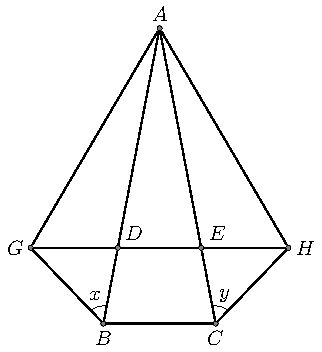
\includegraphics[scale=0.8]{figura}
  \end{minipage}
\end{Problema}

\begin{Solucion}
  
\end{Solucion}

\begin{Problema}{12}
  Se pintan las caras de un cubo, cada una de blanco o negro. �De
  cu�ntas maneras distintas se puede pintar el cubo? (Dos maneras de
  pintar el cubo se consideran iguales si se ven id�nticas girando
  adecuadamente el cubo).
\end{Problema}

\begin{Solucion}
  
\end{Solucion}

\begin{Problema}{13}
  Encuentra el �ltimo d�gito de
  $$
  2012^{(2013^{2014})}- (2012^{2013})^{2014}.
  $$
\end{Problema}

\begin{Solucion}
  
\end{Solucion}

%%% Local Variables: 
%%% mode: latex
%%% TeX-master: "libro"
%%% End: 
